% Chapter 6

\chapter{The critical temperature} % Main chapter title

\label{Chapter6} % For referencing the chapter elsewhere, use \ref{Chapter6} 

\lhead{Chapter 6. \emph{The critical temperature}} % This is for the header on each page - perhaps a shortened title

%----------------------------------------------------------------------------------------
In this chapter we will first derive a linearized gap equation. See section \ref{sec.linearizedgapequation}. This will give us a more efficient way of calculating the critical temperature $T_c$ for the transition between the superfluid and normal phase. In section \ref{sec.criticaltemperature.numerical} we will then solve the equation numerically and investigate the dependency of $T_c$ on the gas parameters $(n_Ba_{BF}^3)^{1/3}$ and $(n_Ba_B^3)^{1/3}$. 

\section{The linearized gap equation} \label{sec.linearizedgapequation}
In the analysis of chapter \ref{Chapter5} the estimation of the critical temperature $T_c$ is quite tedious. We have to wait for an increasing number of iterations near $T_c$ to get a good estimate and calculating the critical temperature as a function of the parameters of the problem is out of the question. In this section we will describe a much more efficient way of estimating the critical temperature through \textit{the linearized gap equation}. This in turn will be performed in section \ref{sec.criticaltemperature.numerical}, where the goal is to calculate the dependency of $T_c$ on the gas parameters.

The gap equation in its full integral form is (see equation \eqref{eq.GapequationIntegral}):
\begin{equation}
\Delta_k = - \int \frac{dk'}{2\pi} W^\text{ind}_{FF}(k,k')\frac{\tanh\left(\frac{\beta E_{F,k}}{2}\right)}{2E_{F,k'}}\Delta_{k'}. \nonumber
\end{equation} 
As we saw in chapter \ref{Chapter5} the gap goes to zero at the critical temperature $T_c$: $\Delta_k(T_c) = 0$. The energy $E_{F,k} = \sqrt{\epsilon_k^2 + |\Delta_k|^2}$ is quadratic in the gap. It follows that by only retaining the gap to first order, we obtain a linear equation near $T_c$:
\begin{equation}
\Delta_k = - \int \frac{dk'}{2\pi} W^\text{ind}_{FF}(k,k')\frac{\tanh\left(\frac{\beta \varepsilon_k}{2}\right)}{2\varepsilon_k} \Delta_{k'}.
\label{eq.GapequationIntegralLinear}
\end{equation} 
Here we have also used, that $\frac{\tanh\left(\frac{\beta \varepsilon_k}{2}\right)}{2\varepsilon_k}$ is even in $\varepsilon_k$, so that the absolute value from the square root can be omitted. This defines a linear equation with eigenvalue $1$: $\Delta_k = L(\Delta_k)$. $L$ is then a linear transformation defined by the integral above. Hence, the program for the evaluation of $T_c$ is now clear. We must find the highest temperature at which, there is an eigenvalue of 1. Notice, that this specifies where the normal to superfluid phase transition occures. This also means, that the chemical potential in $\varepsilon_k = \frac{k^2}{2m_F} - \mu$ can be taken to be the normal phase chemical potential (the chemical potential for the free gas). 

\section{Calculating the critical temperature} \label{sec.criticaltemperature.numerical}
In this section we will describe how in practice to perform the calculation outlined in the above. 

To do the calculation in practice we need to but the linear equation on matrix form. From equation \eqref{eq.GapequationIntegralLinear} it is clear, that we have the matrix equation:
\begin{equation}
\Delta_k = L \Delta_k, \hspace{0.5cm} L(k,k') = -\frac{dk'}{2\pi} W^\text{ind}_{FF}(k,k')\frac{\tanh(\beta \varepsilon_{k'}/2)}{2\varepsilon_{k'}}. 
\label{eq.Gapmatrixequation}
\end{equation}
Explicitly we define a cutoff $k_{\text{up}}$ and spacing $dk'$. We then need to make $k_{\text{up}}$ large enough and $dk'$ small enough for the eigenvalues to have converged. From the form of $L(k,k')$ it is also clear, that $L$ is not a symmetric matrix; each row of $L$ has all the possible values of $\varepsilon_{k'}$, but each column only has a single value belonging to the entire column. The evaluation is performed in MatLab in the following fashion. For a fixed set of parameters we start out with an initial guess $T$ for $T_c$, that we know is too high. We then iteratively decrease $T$ by a small amount $dT$ and calculate the largest eigenvalue for each iteration. When the largest eigenvalue becomes larger than 1, we halt the iteration and set the critical temperature to the current value of $T$. The numerical analysis is a balancing act. We have to choose a resolution fine enough, defined by $dk'$ and $k_{\text{up}}$, for the eigenvalues to have converged to the eigenvalue for the integral operator, and still keep the matrix $L$ small enough for the analysis to be feasible. In this context it is crucial that we have a closed form expression for $W^\text{ind}_{FF}(k,k')$ in the $l_t \to 0$ limit. The analysis is done as previously for a $^{7}\text{Li}$ - $^{40}\text{K}$ mixture. Hence, $m_B/m_F = 7/40$. The ratio of densities is set to $n_F/{n_B^{1/3}} = 0.215$, which means that the boson gas is 100 times denser than the fermion gas. As already commented we use the free gas chemical potential. Since $T/T_F \ll 1$ for all relevant temperatures, we use the Sommerfeld expansion expression: $\frac{\mu(T)}{\epsilon_{F,0}} = 1 + \frac{\pi^2}{12}\left(\frac{T}{T_F}\right)^2$. 

The aboved described strategy is made graphic by figure \ref{fig.TCeigenvalues}. For a specific set of parameters, we have calculated the five highest eigenvalues of $L$ as a function of $T$. We notice, that it is solely the largest eigenvalue, that determines the critical temperature: the eigenvalue crosses 1 for one specific temperature. In the present case: $T_c \approx 0.130 T_F$. The next 4 eigenvalues are significantly lower. 

\begin{figure} 
\begin{center}  
% GNUPLOT: LaTeX picture with Postscript
\begingroup
  \makeatletter
  \providecommand\color[2][]{%
    \GenericError{(gnuplot) \space\space\space\@spaces}{%
      Package color not loaded in conjunction with
      terminal option `colourtext'%
    }{See the gnuplot documentation for explanation.%
    }{Either use 'blacktext' in gnuplot or load the package
      color.sty in LaTeX.}%
    \renewcommand\color[2][]{}%
  }%
  \providecommand\includegraphics[2][]{%
    \GenericError{(gnuplot) \space\space\space\@spaces}{%
      Package graphicx or graphics not loaded%
    }{See the gnuplot documentation for explanation.%
    }{The gnuplot epslatex terminal needs graphicx.sty or graphics.sty.}%
    \renewcommand\includegraphics[2][]{}%
  }%
  \providecommand\rotatebox[2]{#2}%
  \@ifundefined{ifGPcolor}{%
    \newif\ifGPcolor
    \GPcolorfalse
  }{}%
  \@ifundefined{ifGPblacktext}{%
    \newif\ifGPblacktext
    \GPblacktexttrue
  }{}%
  % define a \g@addto@macro without @ in the name:
  \let\gplgaddtomacro\g@addto@macro
  % define empty templates for all commands taking text:
  \gdef\gplbacktext{}%
  \gdef\gplfronttext{}%
  \makeatother
  \ifGPblacktext
    % no textcolor at all
    \def\colorrgb#1{}%
    \def\colorgray#1{}%
  \else
    % gray or color?
    \ifGPcolor
      \def\colorrgb#1{\color[rgb]{#1}}%
      \def\colorgray#1{\color[gray]{#1}}%
      \expandafter\def\csname LTw\endcsname{\color{white}}%
      \expandafter\def\csname LTb\endcsname{\color{black}}%
      \expandafter\def\csname LTa\endcsname{\color{black}}%
      \expandafter\def\csname LT0\endcsname{\color[rgb]{1,0,0}}%
      \expandafter\def\csname LT1\endcsname{\color[rgb]{0,1,0}}%
      \expandafter\def\csname LT2\endcsname{\color[rgb]{0,0,1}}%
      \expandafter\def\csname LT3\endcsname{\color[rgb]{1,0,1}}%
      \expandafter\def\csname LT4\endcsname{\color[rgb]{0,1,1}}%
      \expandafter\def\csname LT5\endcsname{\color[rgb]{1,1,0}}%
      \expandafter\def\csname LT6\endcsname{\color[rgb]{0,0,0}}%
      \expandafter\def\csname LT7\endcsname{\color[rgb]{1,0.3,0}}%
      \expandafter\def\csname LT8\endcsname{\color[rgb]{0.5,0.5,0.5}}%
    \else
      % gray
      \def\colorrgb#1{\color{black}}%
      \def\colorgray#1{\color[gray]{#1}}%
      \expandafter\def\csname LTw\endcsname{\color{white}}%
      \expandafter\def\csname LTb\endcsname{\color{black}}%
      \expandafter\def\csname LTa\endcsname{\color{black}}%
      \expandafter\def\csname LT0\endcsname{\color{black}}%
      \expandafter\def\csname LT1\endcsname{\color{black}}%
      \expandafter\def\csname LT2\endcsname{\color{black}}%
      \expandafter\def\csname LT3\endcsname{\color{black}}%
      \expandafter\def\csname LT4\endcsname{\color{black}}%
      \expandafter\def\csname LT5\endcsname{\color{black}}%
      \expandafter\def\csname LT6\endcsname{\color{black}}%
      \expandafter\def\csname LT7\endcsname{\color{black}}%
      \expandafter\def\csname LT8\endcsname{\color{black}}%
    \fi
  \fi
    \setlength{\unitlength}{0.0500bp}%
    \ifx\gptboxheight\undefined%
      \newlength{\gptboxheight}%
      \newlength{\gptboxwidth}%
      \newsavebox{\gptboxtext}%
    \fi%
    \setlength{\fboxrule}{0.5pt}%
    \setlength{\fboxsep}{1pt}%
\begin{picture}(7200.00,5040.00)%
    \gplgaddtomacro\gplbacktext{%
      \csname LTb\endcsname%
      \put(814,767){\makebox(0,0)[r]{\strut{}$0$}}%
      \csname LTb\endcsname%
      \put(814,1819){\makebox(0,0)[r]{\strut{}$0.5$}}%
      \csname LTb\endcsname%
      \put(814,2872){\makebox(0,0)[r]{\strut{}$1$}}%
      \csname LTb\endcsname%
      \put(814,3924){\makebox(0,0)[r]{\strut{}$1.5$}}%
      \csname LTb\endcsname%
      \put(814,4976){\makebox(0,0)[r]{\strut{}$2$}}%
      \csname LTb\endcsname%
      \put(1009,484){\makebox(0,0){\strut{}$0$}}%
      \csname LTb\endcsname%
      \put(2442,484){\makebox(0,0){\strut{}$0.05$}}%
      \csname LTb\endcsname%
      \put(3875,484){\makebox(0,0){\strut{}$0.1$}}%
      \csname LTb\endcsname%
      \put(5307,484){\makebox(0,0){\strut{}$0.15$}}%
      \csname LTb\endcsname%
      \put(6740,484){\makebox(0,0){\strut{}$0.2$}}%
    }%
    \gplgaddtomacro\gplfronttext{%
      \csname LTb\endcsname%
      \put(176,2871){\rotatebox{-270}{\makebox(0,0){\strut{}$Eigenvalue$}}}%
      \put(3874,154){\makebox(0,0){\strut{}$T/T_F$}}%
    }%
    \gplbacktext
    \put(0,0){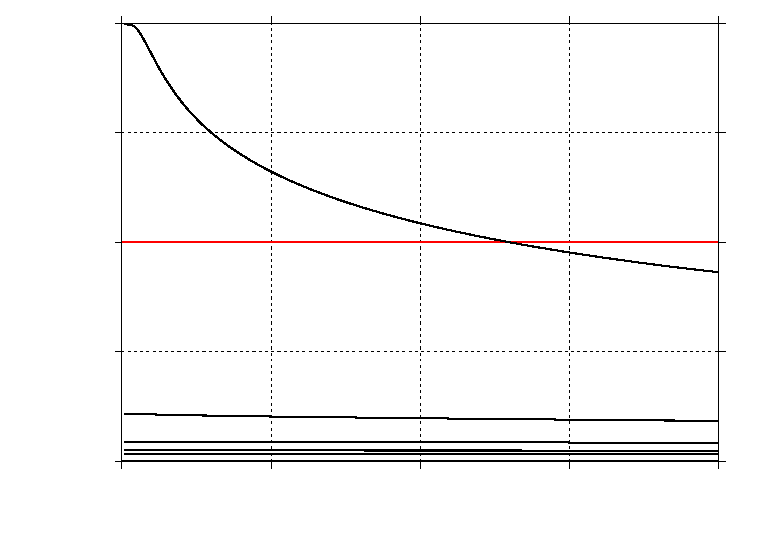
\includegraphics{Figures/TCeigenvalues/TCeigen}}%
    \gplfronttext
  \end{picture}%
\endgroup
  
\caption{In black: The five largest eigenvalues of $L$ plotted as a function of $T$. We see, that the largest eigenvalue intersects 1 (the red line) at one well defined temperature. Parameters: $(n_Ba_{B}^3)^{1/3} = 0.01, (n_Ba_{BF}^3)^{1/3} = 0.1, \frac{m_B}{m_F} = 7/40, \frac{n_F}{n_B^{1/3}} = 0.215$. }
\label{fig.TCeigenvalues}  
\end{center}    
\end{figure}


In figure \ref{fig.TCrB} we see the dependency of $T_c$ on the Bose gas parameter $(n_Ba_B^3)^{1/3}$. We observe a simple monotonic decrease with increasing gas parameter. Physically this can be understood in the following way. When $(n_Ba_B^3)^{1/3}$ is increased for $\frac{n_F}{n_B^{1/3}}$ fixed, the BEC coherence length $k_F\xi = \frac{\pi}{\sqrt{8 n_B/n_F^3 k_Fa_B}}$ decreases. The coherence length is the range of the interaction in real space: $\tilde{V}_{FF}^{\text{ind}} \propto \frac{ \text{e}^{ -\sqrt{2}|x|/\xi } } {|x|}$. Therefore the interaction range is decreased, when we increase $(n_Ba_B^3)^{1/3}$, and so it is physically reasonable, that the critical temperature goes down with increasing $(n_Ba_B^3)^{1/3}$. Notice, that for $(n_Ba_{B}^3)^{1/3} = 0.01$ we recover the critical temperature found in the above: $T_c \approx 0.130 T_F$. 

\begin{figure} 
\begin{center}  
% GNUPLOT: LaTeX picture with Postscript
\begingroup
  \makeatletter
  \providecommand\color[2][]{%
    \GenericError{(gnuplot) \space\space\space\@spaces}{%
      Package color not loaded in conjunction with
      terminal option `colourtext'%
    }{See the gnuplot documentation for explanation.%
    }{Either use 'blacktext' in gnuplot or load the package
      color.sty in LaTeX.}%
    \renewcommand\color[2][]{}%
  }%
  \providecommand\includegraphics[2][]{%
    \GenericError{(gnuplot) \space\space\space\@spaces}{%
      Package graphicx or graphics not loaded%
    }{See the gnuplot documentation for explanation.%
    }{The gnuplot epslatex terminal needs graphicx.sty or graphics.sty.}%
    \renewcommand\includegraphics[2][]{}%
  }%
  \providecommand\rotatebox[2]{#2}%
  \@ifundefined{ifGPcolor}{%
    \newif\ifGPcolor
    \GPcolorfalse
  }{}%
  \@ifundefined{ifGPblacktext}{%
    \newif\ifGPblacktext
    \GPblacktexttrue
  }{}%
  % define a \g@addto@macro without @ in the name:
  \let\gplgaddtomacro\g@addto@macro
  % define empty templates for all commands taking text:
  \gdef\gplbacktext{}%
  \gdef\gplfronttext{}%
  \makeatother
  \ifGPblacktext
    % no textcolor at all
    \def\colorrgb#1{}%
    \def\colorgray#1{}%
  \else
    % gray or color?
    \ifGPcolor
      \def\colorrgb#1{\color[rgb]{#1}}%
      \def\colorgray#1{\color[gray]{#1}}%
      \expandafter\def\csname LTw\endcsname{\color{white}}%
      \expandafter\def\csname LTb\endcsname{\color{black}}%
      \expandafter\def\csname LTa\endcsname{\color{black}}%
      \expandafter\def\csname LT0\endcsname{\color[rgb]{1,0,0}}%
      \expandafter\def\csname LT1\endcsname{\color[rgb]{0,1,0}}%
      \expandafter\def\csname LT2\endcsname{\color[rgb]{0,0,1}}%
      \expandafter\def\csname LT3\endcsname{\color[rgb]{1,0,1}}%
      \expandafter\def\csname LT4\endcsname{\color[rgb]{0,1,1}}%
      \expandafter\def\csname LT5\endcsname{\color[rgb]{1,1,0}}%
      \expandafter\def\csname LT6\endcsname{\color[rgb]{0,0,0}}%
      \expandafter\def\csname LT7\endcsname{\color[rgb]{1,0.3,0}}%
      \expandafter\def\csname LT8\endcsname{\color[rgb]{0.5,0.5,0.5}}%
    \else
      % gray
      \def\colorrgb#1{\color{black}}%
      \def\colorgray#1{\color[gray]{#1}}%
      \expandafter\def\csname LTw\endcsname{\color{white}}%
      \expandafter\def\csname LTb\endcsname{\color{black}}%
      \expandafter\def\csname LTa\endcsname{\color{black}}%
      \expandafter\def\csname LT0\endcsname{\color{black}}%
      \expandafter\def\csname LT1\endcsname{\color{black}}%
      \expandafter\def\csname LT2\endcsname{\color{black}}%
      \expandafter\def\csname LT3\endcsname{\color{black}}%
      \expandafter\def\csname LT4\endcsname{\color{black}}%
      \expandafter\def\csname LT5\endcsname{\color{black}}%
      \expandafter\def\csname LT6\endcsname{\color{black}}%
      \expandafter\def\csname LT7\endcsname{\color{black}}%
      \expandafter\def\csname LT8\endcsname{\color{black}}%
    \fi
  \fi
    \setlength{\unitlength}{0.0500bp}%
    \ifx\gptboxheight\undefined%
      \newlength{\gptboxheight}%
      \newlength{\gptboxwidth}%
      \newsavebox{\gptboxtext}%
    \fi%
    \setlength{\fboxrule}{0.5pt}%
    \setlength{\fboxsep}{1pt}%
\begin{picture}(7200.00,5040.00)%
    \gplgaddtomacro\gplbacktext{%
      \csname LTb\endcsname%
      \put(946,767){\makebox(0,0)[r]{\strut{}$0$}}%
      \csname LTb\endcsname%
      \put(946,1609){\makebox(0,0)[r]{\strut{}$0.05$}}%
      \csname LTb\endcsname%
      \put(946,2451){\makebox(0,0)[r]{\strut{}$0.1$}}%
      \csname LTb\endcsname%
      \put(946,3292){\makebox(0,0)[r]{\strut{}$0.15$}}%
      \csname LTb\endcsname%
      \put(946,4134){\makebox(0,0)[r]{\strut{}$0.2$}}%
      \csname LTb\endcsname%
      \put(946,4976){\makebox(0,0)[r]{\strut{}$0.25$}}%
      \csname LTb\endcsname%
      \put(1141,484){\makebox(0,0){\strut{}$0.005$}}%
      \csname LTb\endcsname%
      \put(2261,484){\makebox(0,0){\strut{}$0.01$}}%
      \csname LTb\endcsname%
      \put(3381,484){\makebox(0,0){\strut{}$0.015$}}%
      \csname LTb\endcsname%
      \put(4500,484){\makebox(0,0){\strut{}$0.02$}}%
      \csname LTb\endcsname%
      \put(5620,484){\makebox(0,0){\strut{}$0.025$}}%
      \csname LTb\endcsname%
      \put(6740,484){\makebox(0,0){\strut{}$0.03$}}%
    }%
    \gplgaddtomacro\gplfronttext{%
      \csname LTb\endcsname%
      \put(176,2871){\rotatebox{-270}{\makebox(0,0){\strut{}$(n_Ba_B^3)^{1/3}$}}}%
      \put(3940,154){\makebox(0,0){\strut{}$T/T_F$}}%
    }%
    \gplbacktext
    \put(0,0){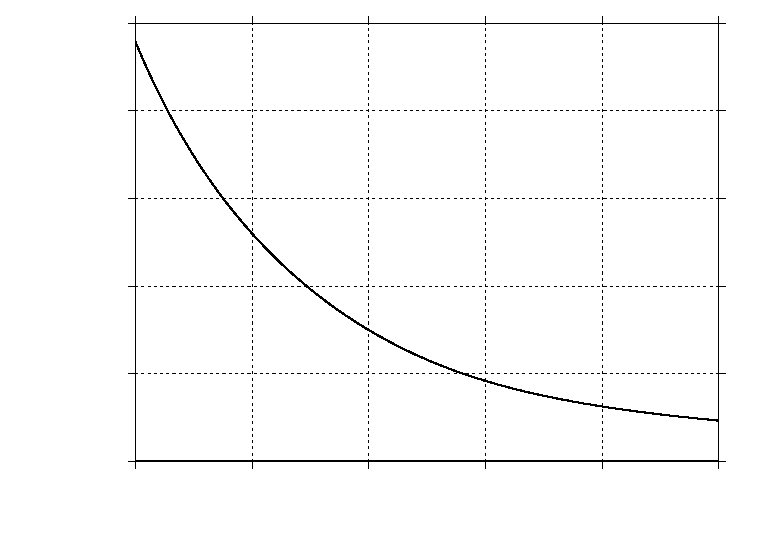
\includegraphics{Figures/TCrB/TCrB}}%
    \gplfronttext
  \end{picture}%
\endgroup
  
\caption{The critical temperatur $T_c$ is plotted as a function of the Bose gas parameter $(n_Ba_B^3)^{1/3}$. We observe a simple monotonic decrease with increasing gas parameter. Other parameters: $(n_Ba_{BF}^3)^{1/3} = 0.1, \frac{m_B}{m_F} = 7/40, \frac{n_F}{n_B^{1/3}} = 0.215$. }  
\label{fig.TCrB}  
\end{center}    
\end{figure}

In figure \ref{fig.TCrBF} we see the dependency of $T_c$ on the Bose-\textit{Fermi} gas parameter $(n_Ba_{BF}^3)^{1/3}$. We observe an increase of $T_c$ with $(n_Ba_{BF}^3)^{1/3}$. This stems from the fact, that a higher value of the Bose-Fermi gas parameter gives a higher interaction strength between the fermions. The system at hand therefore shares one of the key features with the s-wave BCS-theory: any nonzero attractive interaction between the fermions leads to a superfluid phase. 

\begin{figure} 
\begin{center}  
% GNUPLOT: LaTeX picture with Postscript
\begingroup
  \makeatletter
  \providecommand\color[2][]{%
    \GenericError{(gnuplot) \space\space\space\@spaces}{%
      Package color not loaded in conjunction with
      terminal option `colourtext'%
    }{See the gnuplot documentation for explanation.%
    }{Either use 'blacktext' in gnuplot or load the package
      color.sty in LaTeX.}%
    \renewcommand\color[2][]{}%
  }%
  \providecommand\includegraphics[2][]{%
    \GenericError{(gnuplot) \space\space\space\@spaces}{%
      Package graphicx or graphics not loaded%
    }{See the gnuplot documentation for explanation.%
    }{The gnuplot epslatex terminal needs graphicx.sty or graphics.sty.}%
    \renewcommand\includegraphics[2][]{}%
  }%
  \providecommand\rotatebox[2]{#2}%
  \@ifundefined{ifGPcolor}{%
    \newif\ifGPcolor
    \GPcolorfalse
  }{}%
  \@ifundefined{ifGPblacktext}{%
    \newif\ifGPblacktext
    \GPblacktexttrue
  }{}%
  % define a \g@addto@macro without @ in the name:
  \let\gplgaddtomacro\g@addto@macro
  % define empty templates for all commands taking text:
  \gdef\gplbacktext{}%
  \gdef\gplfronttext{}%
  \makeatother
  \ifGPblacktext
    % no textcolor at all
    \def\colorrgb#1{}%
    \def\colorgray#1{}%
  \else
    % gray or color?
    \ifGPcolor
      \def\colorrgb#1{\color[rgb]{#1}}%
      \def\colorgray#1{\color[gray]{#1}}%
      \expandafter\def\csname LTw\endcsname{\color{white}}%
      \expandafter\def\csname LTb\endcsname{\color{black}}%
      \expandafter\def\csname LTa\endcsname{\color{black}}%
      \expandafter\def\csname LT0\endcsname{\color[rgb]{1,0,0}}%
      \expandafter\def\csname LT1\endcsname{\color[rgb]{0,1,0}}%
      \expandafter\def\csname LT2\endcsname{\color[rgb]{0,0,1}}%
      \expandafter\def\csname LT3\endcsname{\color[rgb]{1,0,1}}%
      \expandafter\def\csname LT4\endcsname{\color[rgb]{0,1,1}}%
      \expandafter\def\csname LT5\endcsname{\color[rgb]{1,1,0}}%
      \expandafter\def\csname LT6\endcsname{\color[rgb]{0,0,0}}%
      \expandafter\def\csname LT7\endcsname{\color[rgb]{1,0.3,0}}%
      \expandafter\def\csname LT8\endcsname{\color[rgb]{0.5,0.5,0.5}}%
    \else
      % gray
      \def\colorrgb#1{\color{black}}%
      \def\colorgray#1{\color[gray]{#1}}%
      \expandafter\def\csname LTw\endcsname{\color{white}}%
      \expandafter\def\csname LTb\endcsname{\color{black}}%
      \expandafter\def\csname LTa\endcsname{\color{black}}%
      \expandafter\def\csname LT0\endcsname{\color{black}}%
      \expandafter\def\csname LT1\endcsname{\color{black}}%
      \expandafter\def\csname LT2\endcsname{\color{black}}%
      \expandafter\def\csname LT3\endcsname{\color{black}}%
      \expandafter\def\csname LT4\endcsname{\color{black}}%
      \expandafter\def\csname LT5\endcsname{\color{black}}%
      \expandafter\def\csname LT6\endcsname{\color{black}}%
      \expandafter\def\csname LT7\endcsname{\color{black}}%
      \expandafter\def\csname LT8\endcsname{\color{black}}%
    \fi
  \fi
    \setlength{\unitlength}{0.0500bp}%
    \ifx\gptboxheight\undefined%
      \newlength{\gptboxheight}%
      \newlength{\gptboxwidth}%
      \newsavebox{\gptboxtext}%
    \fi%
    \setlength{\fboxrule}{0.5pt}%
    \setlength{\fboxsep}{1pt}%
\begin{picture}(7200.00,5040.00)%
    \gplgaddtomacro\gplbacktext{%
      \csname LTb\endcsname%
      \put(946,767){\makebox(0,0)[r]{\strut{}$0$}}%
      \csname LTb\endcsname%
      \put(946,1415){\makebox(0,0)[r]{\strut{}$0.02$}}%
      \csname LTb\endcsname%
      \put(946,2062){\makebox(0,0)[r]{\strut{}$0.04$}}%
      \csname LTb\endcsname%
      \put(946,2710){\makebox(0,0)[r]{\strut{}$0.06$}}%
      \csname LTb\endcsname%
      \put(946,3357){\makebox(0,0)[r]{\strut{}$0.08$}}%
      \csname LTb\endcsname%
      \put(946,4005){\makebox(0,0)[r]{\strut{}$0.1$}}%
      \csname LTb\endcsname%
      \put(946,4652){\makebox(0,0)[r]{\strut{}$0.12$}}%
      \csname LTb\endcsname%
      \put(1141,484){\makebox(0,0){\strut{}$0$}}%
      \csname LTb\endcsname%
      \put(2261,484){\makebox(0,0){\strut{}$0.02$}}%
      \csname LTb\endcsname%
      \put(3381,484){\makebox(0,0){\strut{}$0.04$}}%
      \csname LTb\endcsname%
      \put(4500,484){\makebox(0,0){\strut{}$0.06$}}%
      \csname LTb\endcsname%
      \put(5620,484){\makebox(0,0){\strut{}$0.08$}}%
      \csname LTb\endcsname%
      \put(6740,484){\makebox(0,0){\strut{}$0.1$}}%
    }%
    \gplgaddtomacro\gplfronttext{%
      \csname LTb\endcsname%
      \put(176,2871){\rotatebox{-270}{\makebox(0,0){\strut{}$T_c/T_F$}}}%
      \put(3940,154){\makebox(0,0){\strut{}$(n_Ba_{BF}^3)^{1/3}$}}%
    }%
    \gplbacktext
    \put(0,0){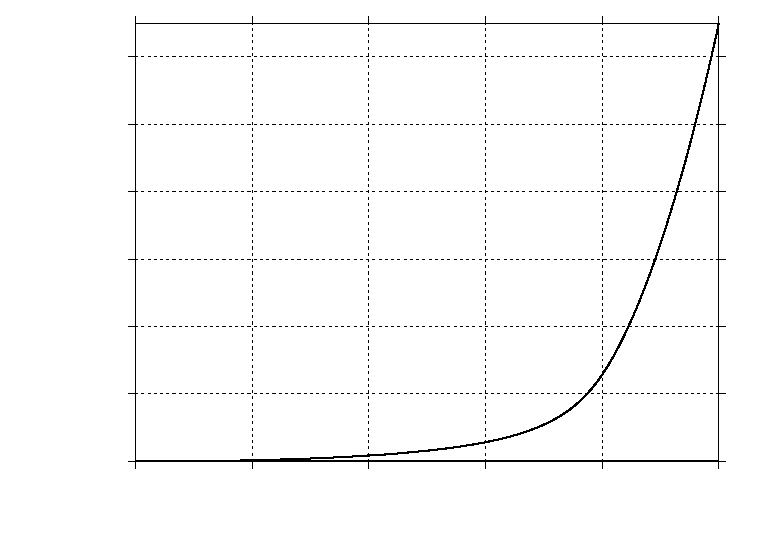
\includegraphics{Figures/TCrBF2/TCrBF}}%
    \gplfronttext
  \end{picture}%
\endgroup
  
\caption{The critical temperatur $T_c$ is plotted as a function of the Bose-Fermi gas parameter $(n_Ba_{BF}^3)^{1/3}$. We see that, for every nonzero induced interaction, that is a superfluid phase for $T\to 0$. Other parameters: $(n_Ba_{B}^3)^{1/3} = 0.01, \frac{m_B}{m_F} = 7/40, \frac{n_F}{n_B^{1/3}} = 0.215$. }  
\label{fig.TCrBF}  
\end{center}    
\end{figure}



